%!TEX root = spack-sc15.tex

\begin{figure}
	\begin{subfigure}{\linewidth}
		\centering
		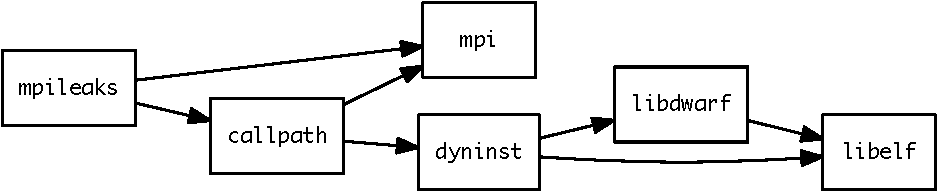
\includegraphics[width=.9\columnwidth]{specs/mpileaks.pdf}
		\caption{
			Spec for {\tt mpileaks}
			\label{fig:specs-mpileaks}
		}
	\end{subfigure}
%
	\begin{subfigure}{\linewidth}
		\centering
		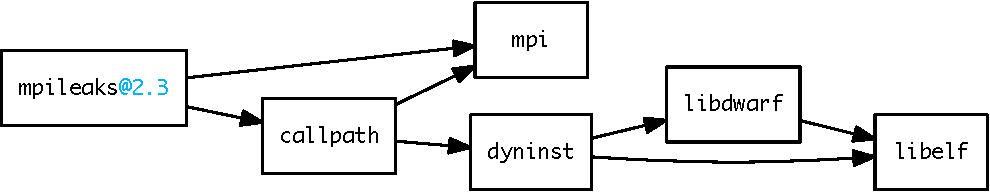
\includegraphics[width=.9\columnwidth]{specs/mpileaks-version}
		\caption{
			{\tt mpileaks@2.3}
			\label{fig:specs-mpileaks-version}
		}
	\end{subfigure}
%
	\begin{subfigure}{\linewidth}
		\centering
		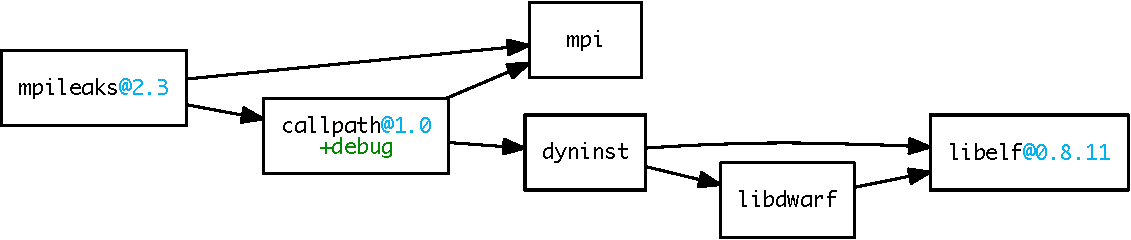
\includegraphics[width=.9\columnwidth]{specs/mpileaks-abstract.pdf}
		\caption{
			{\tt mpileaks@2.3 \^{}callpath@1.0+debug \^{}libelf@0.8.11}
			\label{fig:specs-mpileaks-abstract}
		}
	\end{subfigure}
%
	\caption{
		Constraints applied to {\tt mpileaks} specs.
	}
	\label{fig:specs}
\end{figure}



\subsection{Spack Specs}\label{sec:specs}

Using the simple script in Figure~\ref{fig:mpileaks}, Spack can build many different
versions and configurations of the {\tt mpileaks} package.  In traditional port systems,
package code is structured to build a single version of a package, but in Spack, each
package file is a {\it template} that can be configured and built in many
different ways, according to a set of {\it parameters}.
Spack calls a single build configuration a {\it spec}.
Spack communicates dependencies and parameters to package authors using
the {\tt spec} argument of the {\tt install} method.

\subsubsection{Structure}
To understand specs, consider the {\tt mpileaks} package structure.
Metadata in the {\tt Mpileaks} class (e.g., {\tt version} or
{\tt depends\_on}) describe its relationships with other packages.
The tool has two direct dependencies:
the {\tt callpath} library and {\tt mpi}.  Spack recursively inspects the class definitions
for each dependency and constructs a graph of their relationships.  The result
is a directed, acyclic graph (DAG).\footnote{Spack currently disallows
circular dependencies.}
%
To guarantee a consistent build and to avoid
Application Binary Interface (ABI) incompatibility, we construct
the DAG with only {\it one} version of each package.  Thus, while
Spack can install arbitrarily many configurations of any package,
no two configurations of the same package will ever appear in the same build DAG.

DAGs for {\tt mpileaks} are shown in Figure~\ref{fig:specs}.
Each node represents a package, and each package has five configuration parameters that control
how it will be built: 1) the package version, 2) the compiler with which to
build, 3) the compiler version, 4) named compile-time build options, or
{\it variants}, and 5) the target architecture.


\subsubsection{Configuration Complexity}
A spec DAG has many degrees of freedom, and users cannot reasonably be
expected to understand or to specify all of them.  In our experience at LLNL,
the typical user only cares about a small number of build constraints (if any),
and does not know enough to
specify the rest. For example, a user may know that a certain version of a library like
{\tt boost}~\cite{boost} is required, but only cares that other build parameters are set so that
the build will succeed.
%
Configuration complexity makes the HPC software ecosystem difficult to manage:
too many parameters exist to specify them all. However, the known and
important ones often provide detailed build constraints. Thus, we have two
competing concerns.  We need the ability to specify details
without having to remember all of them.

\subsubsection{Spec Syntax}\label{sec:syntax}
\begin{figure}
{\fontfamily{cmr}\selectfont
\begin{grammar}\small
  <spec>         ::= <id> [ <constraints> ]

  <constraints>   ::= \{ `@' <version-list> | `+' <variant> \newline
                   | `-' <variant> ~~~| `~' <variant> \newline
                   | `\%' <compiler> ~| `=' <architecture> \} \newline
                  [ <dep-list> ]

  <dep-list>  ::= \{ `\textsf \textasciicircum' <spec> \}

  <version-list> ::= <version> [ \{ `,' <version> \} ]

  <version>      ::= <id> | <id> `:' | `:' <id> | <id> `:' <id>

  <compiler>     ::= <id> [ <version-list> ]

  <variant>      ::= <id>

  <architecture> ::= <id>

  <id>           ::= "[A-Za-z0-9_][A-Za-z0-9_.-]*"
\end{grammar}
} % End fontfamily{cmr}
\caption{
	EBNF grammar for spec expressions.
	\label{fig:grammar}
}
\end{figure}


\begin{table*}\centering
\begin{tabular}{|r|p{2.4in}|p{4in}|}
\hline
& {\bf Spec} & {\bf Meaning} \\
\hline
\hline
1&\small\verb|mpileaks|                         & \small {\tt mpileaks} package, no constraints. \\\hline
2&\small\verb|mpileaks@1.1.2|                   & \small {\tt mpileaks} package, version 1.1.2. \\\hline
3&\small\verb|mpileaks@1.1.2 %gcc|              & \small {\tt mpileaks} package, version 1.1.2, built with {\tt gcc} at the default version. \\\hline
4&\small\verb|mpileaks@1.1.2 %intel@14.1 +debug| & \small {\tt mpileaks} package, version 1.1.2, built with Intel compiler version 14.1, \newline with the ``debug'' build option. \\\hline
5&\small\verb|mpileaks@1.1.2 =bgq|              & \small {\tt mpileaks} package, version 1.1.2, built for the Blue Gene/Q platform (BG/Q). \\\hline
6&\small\verb|mpileaks@1.1.2 ^mvapich2@1.9|     & \small {\tt mpileaks} package version 1.1.2, using {\tt mvapich2}  version 1.9 for MPI. \\\hline
7&\small\verb|mpileaks @1.2:1.4 %gcc@4.7.5 -debug =bgq| \newline
      \verb|  ^callpath @1.1 %gcc@4.7.2| \newline
      \verb|  ^openmpi @1.4.7|                & \small%
      {\tt mpileaks} at any version between 1.2 and 1.4 (inclusive), built with gcc 4.7.5,
      without the debug option, for BG/Q, linked with {\tt callpath} version 1.1
      and building {\tt callpath} with {\tt gcc} version 4.7.2, linked with {\tt openmpi} version 1.4.7.    \\
\hline
\end{tabular}
\caption{
	Spack build spec syntax examples and their meaning.
	\label{tab:specs}
}
\end{table*}

We have developed a syntax for specs that allows users to specify
only constraints that matter to them. Our syntax can represent
DAGs concisely enough for command line use.
The spec syntax is recursively defined to allow users to specify
parameters on dependencies as well as on the root of the DAG.
Figure~\ref{fig:grammar} shows the EBNF grammar through which Spack
flexibly supports constraints.

We begin with a simple example.
Consider the case where a user wants to install the {\tt mpileaks} package, but knows
nothing about its structure.  To install the package, the user invokes {\tt spack install}:
%
\begin{minted}[fontsize=\scriptsize]{bash}
    $ spack install mpileaks
\end{minted}
%
Here, {\tt mpileaks} is the simplest possible spec---a single identifier.
Spack converts it into the DAG shown in Figure~\ref{fig:specs-mpileaks}.
Note that even though the spec contains no dependency information, it is still
converted to a full DAG, based on directives supplied in package files. Since
the spec does not constrain the nodes, Spack has leeway when building the
package, and we say that it is {\it unconstrained}.
%
However, a user who wants a specific {\tt mpileaks} version can
request it with a version constraint after the package name:
%
\begin{minted}[fontsize=\scriptsize]{bash}
    $ spack install mpileaks@2.3
\end{minted}
%
Figure~\ref{fig:specs-mpileaks-version} shows that the specific version
constraint is placed on the {\tt mpileaks} node in the DAG, which otherwise
remains unconstrained.
A user who only requires a particular minimum version could use
{\it version range} syntax
and write {\tt @2.3:}.  Likewise, {\tt @2.3:2.5.6} would specify a
version between 2.3 and 2.5.6. In these cases, the user can save time if
Spack already has a version installed that satisfies the spec -- Spack will use
the previously-built installation instead of building a new one.

Figure~\ref{fig:specs-mpileaks-abstract} shows the recursive nature of the spec syntax:
%
\begin{minted}[fontsize=\scriptsize]{bash}
    $ spack install mpileaks@2.3 ^callpath@1.0+debug ^libelf@0.8.11
\end{minted}
%
The caret (\verb|^|) denotes constraints for a particular dependency. The DAG
now has version constraints on {\tt callpath} {\it and} {\tt libelf},
and the user has requested the {\tt debug} variant of the {\tt callpath} library.

Recall that Spack guarantees that only a single version of any package occurs
in a spec.  Within a spec, each dependency can be uniquely
identified by its package name alone.  Therefore, the user does not need to consider
DAG connectivity to add constraints but instead must only know that
{\tt mpileaks} depends on {\tt callpath}.
Thus, dependency constraints can appear in an arbitrary order.

Table~\ref{tab:specs} shows further examples of specs, ranging from
simple to complex. These examples show how Spack's constraint
notation covers the rest of the HPC package parameter space.

{\bf Versions.}
Version constraints are denoted with {\tt @}. Versions
can be precise ({\tt @2.5.1}) or denote a range ({\tt @2.5:4.4}),
which may be open-ended ({\tt @2.5:}).
%
The package in Figure~\ref{fig:mpileaks} lists two ``safe'' versions with
checksums, but
in our experience users frequently want bleeding-edge versions, and package managers
often lag behind the latest releases.
Spack can extrapolate URLs from versions,
using the package's {\tt url} attribute as a model.\footnote{This works
for packages with consistently named URLs.}  If the user requests a specific
version on the command line that is unknown to Spack,
Spack will attempt to fetch and to install it.  Spack uses the same
model to scrape webpages and to find new versions as they become available.

\begin{figure}
\begin{minted}[linenos,
               numbersep=5pt,
			   fontsize=\scriptsize,
               frame=lines,
               framesep=2mm]{python}
    def install(self, spec, prefix):  # default build uses cmake
        with working_dir('spack-build', create=True):
            cmake('..', *std_cmake_args)
            make()
            make("install")

    @when('@:8.1')                    # <= 8.1 uses autotools
    def install(self, spec, prefix):
        configure("--prefix=" + prefix)
        make()
        make("install")
\end{minted}
\caption{
    Specialized {\tt install} method in Dyninst.
	\label{fig:specialization}
}
\end{figure}

{\bf Compilers.}
With a compiler constraint (shown on line 3) the user
simply adds {\tt \%} followed by its name, with an optional compiler version
specifier.  Spack compiler names like {\tt gcc} refer to the full compiler {\it toolchain},
i.e., the C, C++, and Fortran 77 and 90 compilers.  Spack can auto-detect
compiler toolchains in the user's {\tt PATH}, or they can be registered manually
through a configuration file.

{\bf Variants.}
To handle options like compiler flags or optional components, specs can
have named flags, or {\it variants}.  Variants are associated with the package,
so the {\tt mpileaks} package implementer must explicitly handle cases
where debug is enabled ({\tt +debug}) or disabled ({\tt -debug}
or {\tt \textasciitilde \ignorespaces debug}).  Names simplify versioning
and prevent the configuration space from becoming too large.
For example, including detailed compiler flags in spec syntax
would violate our goal of conciseness, but known sets of flags can simply be named.

{\bf Cross-compilation.}
To support cross-compilation, specs can include the system architecture
(line 5). Platforms begin with {\tt =} and take names like {\tt linux-ppc64}
or {\tt bgq}.  They are specified per-package. This mechanism allows front-end
tools to depend on their back-end measurement
libraries with a {\it different} architecture on cross-compiled machines.

\subsubsection{Constraints in Packages}\label{sec:constraints}

So far, we have shown examples of specs used to request constraints from the
command line, when {\tt spack install} is invoked.  However, the user is not
the only source of constraints.  Applications may require specific versions
of dependencies. Often, these constraints should be specified in a package
file.  For
example, the ROSE compiler~\cite{rose} only builds with a certain version of the {\tt boost} library.
The {\tt depends\_on()} directives in Figure~\ref{fig:mpileaks} contain
simple package names.  However, a package name is also a spec, and
the same constraint syntax usable from the command line can be applied inside directives.
So, we can simply write:
%
\begin{minted}[fontsize=\scriptsize]{python}
    depends_on('boost@1.54.0')
\end{minted}
%
This constraint will be incorporated into the initial DAG node generated from
the {\tt ROSE} package.  Dependencies can also be {\it conditional}.  For example,
the {\tt ROSE} package builds with different versions of boost, depending on the
compiler version. So, directives also accept spec syntax as a
predicate in an optional {\tt when} parameter:
%
\begin{minted}[fontsize=\scriptsize]{python}
    depends_on('boost@1.47.0', when='%gcc@:4')
    depends_on('boost@1.54.0', when='%gcc@5:')
\end{minted}
%
\vfill\eject
\noindent
The same notation is used to build optionally with libraries like MPI:
%
\begin{minted}[fontsize=\scriptsize]{python}
    depends_on('mpi', when='+mpi')
\end{minted}
%
and to ensure that specific patches are applied to Python source code
when it is built on Blue Gene/Q, with different compilers:
%
\begin{minted}[fontsize=\scriptsize]{python}
    patch('python-bgq-xlc.patch',   when='=bgq%xl')
    patch('python-bgq-clang.patch', when='=bgq%clang')
\end{minted}
%
Constraints in the {\tt when} clause are matched against the package spec.
Outside of directives, constraints can also be tested directly on the {\tt spec}
object in the {\tt install} method:
%
\begin{minted}[fontsize=\scriptsize]{python}
  def install(self, spec, prefix):
      if spec.satisfies('%gcc'):
          # Handle gcc
      elif spec.satisfies('%xl'):
          # Handle XL compilers
\end{minted}
%

\subsubsection{Build Specialization}

In our experience maintaining packages at LLNL, we often must change
entire package build scripts due to large changes in the way certain packages build.
These changes are cumbersome, particularly since we often must maintain both
the old and new version of a build script, as some users rely on the old version.


%class Dyninst(Package):
%    """"Dyninst binary instrumentation and analysis tool."""
%    url="http://www.paradyn.org/release8.1/DyninstAPI-8.1.1.tgz"
%    version('8.1.1', 'd1a04e995b7aa70960cd1d1fac8bd6ac')
%    depends_on("libelf")
%    depends_on("libdwarf")
%    depends_on("boost@1.42:")
%

Spack provides functionality that allows Python functions to have
multiple definitions, each specialized for particular configurations of the package.
This capability allows us to have two separate implementations of {\tt install} or {\it any} method
in a package class, as Figure~\ref{fig:specialization} shows for the Dyninst
package.  The {\tt @when} directive is a Python decorator: a higher order function that
takes a function definition as a parameter and returns a new function to replace it.
We replace the function with a callable multi-function dispatch object, and we
integrate the predicate check into the function dispatch mechanism.  The
{\tt @when} condition is true when Dyninst is at version 8.1 or lower, in which
case the package will use the {\tt configure}-based build.  By default if no predicate matches,
{\tt install} will use the default CMake-based implementation. The simple {\tt @when}
annotation allows us to maintain our old build code alongside the new version without
accumulating complex logic in a single {\tt install} function.
